\pagestyle{empty}
\cleardoublepage
\pagestyle{fancy}

\chapter{Modelagem Eletromagnética do Mancal}

%Passos da modelagem:
%
%\begin{enumerate}[a.]
%	\item modelagem eletromagnética da parte passiva $\rightarrow$ Força passiva dependente de x,y,z
%	\item modelagem eletromagnética da parte ativa  $\rightarrow$ Força ativa de pedente de x,y,z,i
%	\item fundir modelos
%	\item modelagem da dinâmica e acoplamentos 
%\end{enumerate}

%Dimensões do mancal (Fig. \ref{Fig:Modelagem:Dimensoes})

Abordaremos nesse capítulo a modelagem eletromagnética do mancal magnético proposto, essa etapa é importante para o entendimento das influências dos parâmetros geométricos no circuito eletromagnético além de possibilitar a criação de um modelo realista das forças atuantes no rotor. Com o equacionamento das forças um modelo inicial em elementos finitos foi criado e simulações realizadas para a obtenção de um melhor modelo. 

As nomenclaturas das dimensões a serem utilizadas nas seguintes secções para modelagen e parametrização do sistema são ilustradas na Fig. \ref{Fig:Modelagem:Dimensoes}.

\begin{figure}[!ht]
	\centering
	\def\svgwidth{\columnwidth}
	\includesvg{modelo:dim}
		\caption{Dimensões do mancal}
		\label{Fig:Modelagem:Dimensoes}
\end{figure} 

\section{Circuito passivo}

A parte passiva do mancal magnético pode ser descrita como o circuito da Fig. \ref{Fig:Modelagem:circuito:passivo:umlado}, onde um ímã permanente gera um fluxo magnético que estabiliza o eixo axial (passivo), o caminho principla desse fluxo atravessa o entreferro tanto pelos ferros do estator quanto pelo do rotor. Dois caminhos extras são considerados, um de fuga de fluxo magnético no ímã e outro no entreferro. 

\begin{figure}[!ht]
	\centering
	\def\svgwidth{1\columnwidth}
	\includesvg{modelo:circuito:passivo:umlado}
	\caption{Circuito magnético passivo suposto}
	\label{Fig:Modelagem:circuito:passivo:umlado}
\end{figure}

\todo[inline]{descrever mais ??}

Sendo:
\begin{itemize}
	\item $\mathcal{F}_c$ :  Força magnética coerciva;
	\item $\phi_m$ : Fluxo magnético que atravessa o ímã;
	\item $\phi_f$ : Fluxo magnético no circuíto principal;
	\item $\phi_g$ : Fluxo magnético que atravessa o entreferro;
	\item $\phi_{lm}$ : Fluxo magnético de fuga no ímã;
	\item $\phi_{lg}$ : Fluxo magnético de fuga no entreferro;
	\item $\mathcal{R}_m$ : Relutância magnética do ímã;
	\item $\mathcal{R}_{lm}$ : Relutância magnética de fuga no ímã;
	\item $\mathcal{R}_{fef}$ : Relutância magnética no ferro estator;
	\item $\mathcal{R}_{ge}$ : Relutância magnética no entreferro;
	\item $\mathcal{R}_{lg}$ : Relutância magnética de fuga no entreferro;
	\item $\mathcal{R}_{rf}$ : Relutância magnética no ferro do rotor;
	\item $\mathcal{R}_{lg}$ : Relutância magnética no retorno do rotor;
\end{itemize}

\subsection{Premissas}

Nesse modelo, o ímã é considerado como uma fonte de fluxo magnético na forma equivalente de um circuito Thevenin. A força magnética coerciva ($\mathcal{F}_c$) representa a força magnética necessária para impor o ímã permanente a produzir um fluxo magnético nulo. Ímãs de terra rará (Samário Cobalto - Neodímio), possuem tipicamente uma curva linear de magnetização no segundo quadrante, essa curva depende de duas constantes físicas do material usado: $H_c$ uma constante que associa o comprimento do ímã com a força coerciva ($ F_c = H_c \, l_m$) e $B_r$ que descreve o fluxo máximo do ímã num cenário de curto circuíto ($\phi_r = B_r \, A_m$), a descrita é ilustrada na Fig. \ref{Fig:Modelagem:circuito:passivo:ima}.

\begin{figure}[!ht]
	\centering
	\def\svgwidth{0.7\columnwidth}
	\includesvg{modelo:circuito:passivo:ima}
	\caption{Curva de desmagnetização típica de ímãs de terra rará}
	\label{Fig:Modelagem:circuito:passivo:ima}
\end{figure}

A curva de magnetização pode ser descrita como :

\begin{align}
	B_m = B_r + \frac{B_r}{H_c} H_m
	\label{eq:p:ima}
\end{align}

A relação $\frac{B_r}{H_c}$ pode ser interpretada como a permeabilidade do meio (ímã) e é tipicamente próxima a $\mu_0$. O ponto de operação do ímã depende da curva de carga do circuíto magnético em que ele está inserido, para isso é necessário primeiramente calcular o valor da permeabilidade total e então identificar o ponto de operação do ímã e o seu fluxo produzido.

Considera-se nesse modelo para os materiais ferros magnéticos a curva de magnetização do ferro 1020 (\ref{} \todo{ref. tab}), a curva não linear é apresentada na Fig. \ref{Fig:Modelagem:BH}, nota-se que a saturação ocorre por volta de 1.3T. Essa relação pode ser descrita como :

\begin{align}
	B(H) = \mu(H) \, H
	\label{eq:p:BH:ferro}
\end{align}


\begin{figure}[!ht]
\centering
	\caption*{ Vetor campo magnético (T) x Campo Magnético (A/m)}
 	\includegraphics[width=0.6\linewidth]{modelo:curva:BH}
	\caption{Curva de magnetização para o ferro 1020}
	\label{Fig:Modelagem:BH}
\end{figure}


\subsection{Campo magnético no entreferro}

A relutância magnética é proporcional ao comprimento da linha de campo no meio e inversamente proporcional a permeabilidade do meio e a área. Com isso, calcula-se as relutância principais do circuíto :

\begin{align}
	 R_{p}  &= \frac{h_m}{\mu_m \, S_m}			\\
	 R_{ef} &= \frac{w_{ef}}{\mu_{ef}\, S_{ef}}  \\     
	 R_{rf} &= \frac{w_{rf}}{\mu_{rf}\, S_{rf}}   \\    
	 R_{rr} &= \frac{h_m}{\mu_{rr} \, S_{rr}}     \\      
	 R_{ge} &= \frac{l_g}{\mu_0  \, S_{ge}}        
\end{align}

A permeância gerada pelo vazamento podem ser calculadas por \ref{}  :
\begin{align}
	P_{lm} &= \frac{0.64 \,  \mu_0 \,r_{ee}}{h_m/(h_m+2h_{ef})+1} \\
	R_{lg} &= P_1 + P_2 + P_3 + P_4	
\end{align} \todo{colocar anexo}

Sendo $R_{g//}$ a associação paralela entre a relutância do entreferro e o vazamento associado, $R_1$ a soma das relutâncias do circuíto principal e $R_T$ a associação entre as relutâncias dos circuítos 1 e 2. Obtém-se as equações:

\begin{align}
	\phi_m &= \phi_1 + \phi_2 \\
		   &= \frac{F_c}{R_p + R_T} \\
	F_c	   &= \phi_1 \, (R_p + R_1) \\
	F_c    &= \phi_2 \, (R_p + R_{lm})
\end{align}

Encontra-se o campo magnético efetivo no entreferro :

\begin{align}
   \phi_{ge} &= \frac{\phi_1 \, R_{lg}}{R_{ge}+R_{lg}} \\
   B_{ge} &= \frac{\phi_g}{S_{ge}}
\end{align}

\subsubsection{Convergência}

Como a permeabilidade de materiais ferros magnéticos variam com o campo magnético, é preciso realizar uma série de interações para alcançar a convergência do valor do campo magnético nas partes do circuíto. 

Nesse caso atribui-se um valor inicial para a permeabilidade nos três componentes do circuíto (ferro estator, ferro rotor e ferro retorno), aplicando esses valores para o cálculo do campo magnético no entreferro obtém-se novos valores do campo magnético nesses mesmos componentes, é então derivado os valores para a permeabilidade através de uma interpolação linear. Calcula-se então os novos valores da próxima interação pelo método de Newton-Raphson \ref{}. A Fig. \ref{fig:passivo:convergencia} ilustra a analise da convergência dos resultados para uma determinada configuração de parâmetros construtivos.  

%\begin{figure}[ht!]
%\centering
%\caption*{Vetor campo magnético (B) vs Interações}
%\includegraphics[width=0.6\linewidth]{./Simulacoes/Passivo2/passivo:convergencia}
%\caption{Análise de convergência do vetor campo magnético no entreferro}
%\label{fig:passivo:convergencia}
%\end{figure}

%\subsection{Validação}
%
%O resultado obtido com o modelo magnético analítico é confrontando com os resultados obtidos 


\subsection{Decomposição do campo magnético B em X e Z} \label{SubSec:CampoX/Y}

O campo magnético acumulado no entreferro pode ser decomposto em componentes $B_x$ e $B_z$ que dependem do deslocamento do rotor em $\Delta_x$ e $\Delta_z$, esse deslocamento implica também em um aumento no comprimento do gap: $l_g$, A Fig. \ref{Fig:modelo:passivo:DxDz} ilustra o deslocamento. Tal modelo não leva en consideração o \textit{tilt} do rotor, que implicaria em relutâncias diferentes para a parte superior e inferior do rotor. 

	\begin{figure}[!ht]
		\centering
		\def\svgwidth{0.6\columnwidth}
		\includesvg{modelo:passivo:DxDy}
			\caption{Deslocamento em X e Y}
			\label{Fig:modelo:passivo:DxDz}
	\end{figure}

 Os campos podem então ser derivados:
 
 \begin{align}
 	\theta_z &= tg^{-1}(\frac{\Delta_z}{\Delta_x}) \\
 	l_g &= \sqrt{\Delta_x^2 + \Delta_z^2} \\
 	B_{gx} &= B \, cos(\theta_z) \\
 	B_{gz} &= B \, sin(\theta_z) 
 \end{align}


\subsection{Força}

A força magnética de atração do rotor pelo estator é gerada pela energia eletromagnética acumulada no entreferro (superior e inferior), essa força pode então ser calculada através do trabalho virtual \citep{Chiba}:

\begin{align}
	|\vec{F}(l_g)| &= 2 \, \frac{ \vec{B}_{g}^2 \; S_g}{2 \, \mu_0} \label{eq:passivo:Fx}
\end{align}

\subsubsection{Força radial} \label{subsection:forca:x}


Desejamos obter as resultantes das forças projetadas nos eixos radiais (x e y), para obtermos um modelo mais preciso das forças, o mancal foi divido em oito partes distintas sendo que cada parte possui um componente de campo magnético diferente das outras partes. Para então obtermos o valor das forças radiais, precisamos calcular todas as forças e então decompor-las nos eixos (Fig. \ref{Fig:Modelagem:circuito:passivo:forca}). Por inspeção :

\begin{align}
	F_x &= F_{L} + F_{NL} \, \boldsymbol{i} + F_{SL} \, \boldsymbol{i} - F_{O} - F_{NO} \, \boldsymbol{i}  - F_{SO} \, \boldsymbol{i} \label{eq:p:F:resultante:x} \\
	F_y &= F_{N} + F_{NL} \, \boldsymbol{j} + F_{SL} \, \boldsymbol{j} - F_{S} - F_{NO} \, \boldsymbol{j}  - F_{SO} \, \boldsymbol{j}
	\label{eq:p:F:resultante:y} 
\end{align}

Onde $\boldsymbol{i}$ é a projeção da força no eixo x e $\boldsymbol{j}$ é a projeção da força no eixo y. Para pequenos deslocamentos (Fig. \ref{fig:Passivo:gap}), a variação no ângulo $\theta$ pode ser desprezível e sempre ser considerado como $45$ graus.

%\[
%\theta_{NO} = \tan \left(\frac{r_{eei} - g_{eN}}{r_{eei} - g_{eO}} \right)
%\]

\[
\theta_{NO} = 45^{\circ}
\]

 	\begin{figure}[!ht]
 		\centering
			\includesvg{modelo:circuito:passivo:gap}
 			\caption{Decomposição de força passiva para uma determinada secção}
 			\label{fig:Passivo:gap}
 	\end{figure}

%portanto:

%\begin{align}
%	F_{NL} \, \boldsymbol{i} &= F_{NL}(G_{eNO}) \, \cos (^{\circ}) \\
%	F_{NL} \, \boldsymbol{j} &= F_{NL}(G_{eNO}) \, \sin (\theta_{NO}) 
%\end{align}

%\begin{align}
%	F_{NL} \, \boldsymbol{i} &= F_{NL}(G_{eNO}) \, \frac{1}{\sqrt{2}} \\
%	F_{NL} \, \boldsymbol{j} &= F_{NL}(G_{eNO}) \, \frac{1}{\sqrt{2}}
%\end{align}
%
%E similarmente para as outras forças.
%
%\begin{align}
%	F_{NL}
%\end{align}

\subsubsection{Força axial}

A força perpendicular ao plano de rotação é a composição de todos os oito segmentos, não é levado em consideração o efeito de tilt do rotor. Obtemos:

\begin{equation}
	  		F_z(l_g) = \frac{S_{g}}{2 \, \mu_0} 	\sum_{i=N}^{NO} B_{giz}^2
\end{equation}

\subsection{Validação do modelo}

O modelo obtido analiticamente é contrastado com o um em elementos finitos desenvolvido em três dimensões, aplicou-se a ambos os modelos as mesmas constantes magnéticas (permeabilidade, curva B-H) e parâmetros geométricos/construtivos.

Os resultados obtidos em ambos os modelos são comparados a seguir.


\begin{figure}[th!]
\centering
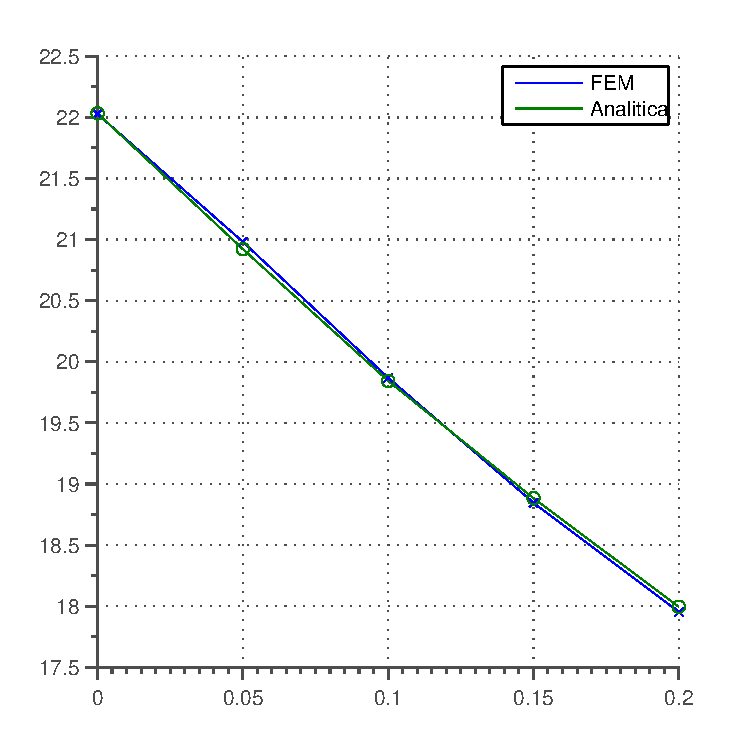
\includegraphics[width=0.7\linewidth]{Simulacoes/Passivo2/validacao_passivo_dx_calibrado}
\caption{}
\label{fig:validacao_passivo_dx_calibrado}
\end{figure}




\subsection{Otimização dos parâmetros}

Buscou-se uma combinação de parâmetros que maximizasse a força de atração axial e que minimizasse a força longitudinal. O mancal deve possuir rigidez suficiente para suspender o conjunto inércia, rotor mancal, rotor motor. Estudos realizados estimam um momento de inércia total para o sistema de $6.9 \, 10^{-2} \, kg \, m^2$ com uma massa de 3.52 kg (para operar em ambiente com gravidade). 



%\subsection{Escolha dos parâmetros}
%
%Buscou-se uma combinação de parâmetros que maximizasse a força de atração axial e que minimizasse a força longitudinal.  As áreas e comprimentos médios são obtidos da seguinte maneira (com uma zona de integração de $45^{\circ}$), com referência a Fig. \ref{Fig:Modelagem:Dimensoes} e a tabela em Anexo \ref{Tabela:Modelagem:Dimensoes}
%
%\begin{align}
%	S_m &= w_m     	\frac{2 \pi (r_{eei} + w_{fee} - w_m)}{8} \\
%	S_f &= h_{fee} 	\frac{2 \pi r_{eei}}{8} \\
%	S_g(l_g) &= h_{fee}	\frac{2 \pi (r_{reei} - \nicefrac{l_g}{2})}{8} \alpha_g \\
%	l_m &= h_m \\
%	l_f &= w_{fee}
%\end{align}
%
%%\todo[inline]{Explicar melhor o que é espraiamento e como encontrar-lo}
%
%O termo $ \alpha_g $ é o fator de espraiamento do campo magnético no entreferro do mancal  que é devido a dispersão do campo magnético, ou seja a área em que o entreferro acumula campo magnético é sempre maior ($\alpha_g > 1)$ do que a área calculada.  
%
%Podemos calcular o acréscimo de área devido ao  espraiamento  (\citet{Leupold1990}) como sendo dependente do tamanho do entreferro e da geometria, podemos assumir como aproximação que o espraiamento é regido pela seguinte equação:
%
%\begin{align}
%	P = 0.318 ln \left( 1 + \frac{2 w}{g} \right)
%	\label{eq:passivo:p}
%\end{align}
% 
%\begin{figure}[th!]
%\centering
%\includegraphics[width=0.3\linewidth]{./Figs/modelo:passivo:espraiamento}
%\caption{Cálculo do fator de espraiamento}
%\label{fig:modelo:passivo:espraiamento}
%\end{figure}
%
%O mancal deve possuir rigidez suficiente para suspender o conjunto inércia, rotor mancal, rotor motor. Estudos realizados estimam um momento de inércia total para o sistema de $6.9 \, 10^{-2} \, kg \, m^2$ com uma massa de 3.52 kg (para operar em ambiente com gravidade). 
%
%\subsection{Simulações}
%
%Simulações foram realizados com o intuito de classificar as forças atuantes no rotor devido ao circuito magnético do estator externo. As simulações foram realizadas utilizando os parâmetros construtivos em da Tabela em Anexo \cite{Anexo}.
%
% Verificamos na Fig. \ref{fig:forca:passivo:fx:modelagem:diff} a simulação da translação do rotor em apenas um dos eixos radiais, podemos verificar a linearidade da força quando o rotor trabalha em modo diferencial.  O máximo deslocamento é limitado em $0,35$mm pelo efeito do batente.
%
%\begin{figure}[!ht]
%\centering
%\caption*{Força (N) x $\Delta_x$ (mm) - Deslocamento Radial: y = 0, z = 0}
%\includegraphics[width=0.6 \columnwidth,angle=0]{Figs/Simulacoes/Passivo/forca:fx:passivo:modelagem}
%\caption{Força atuante no rotor dado uma translação radial}
%\label{fig:forca:passivo:fx:modelagem:diff}
%\end{figure}
%
%
%Um mapa  do módulo da força radial no plano x,y é ilustrado na Fig. \ref{fig:forca:passivo:mod:fx:fy:3d}, notamos que em torno do ponto de operação a força é praticamente nula. Porém quando o rotor encontra-se em algum de seus extremos, a força de atração é da ordem de centenas de Newton o que vai influenciar na definição do circuito ativo que tem que ser capaz de vencer essa força.
%
%\begin{figure}[!ht]
%\centering
%\caption*{Módulo Força (N) x Deslocamento (mm)}
%\includegraphics[width=0.8\linewidth]{./Figs/Simulacoes/Passivo/forca:passivo:mod:fx:fy:3d}
%\caption{}
%\label{fig:forca:passivo:mod:fx:fy:3d}
%\end{figure}
%
%A força devido a translação axial é ilustrado na Fig. {fig:forca:passivo:fz:centro}, essa força restaurativa torna a parte passiva do mancal estável e é a responsável pela rigidez nesse grau de liberdade. Notamos que a força necessária para deslocar 1mm axialmente quando o mancal está no ponto de operação é de aproximadamente 850N.
%
%%\begin{figure}[!ht]
%%\centering
%%\caption*{Força (N) x $\Delta_z$ (mm) - Deslocamento Axial: x = 0, y = 0}
%%\includegraphics[width=0.6 \columnwidth,angle=0]{Figs/Simulacoes/Passivo/forca:passivo:fz:centro}
%%\caption{Força atuante no rotor dado uma translação axial}
%%\label{fig:forca:passivo:fz:centro}
%%\end{figure}
%
%\subsection{Elementos Finitos}
%
% O módulo do campo magnético pode ser visualizado para dois casos distintos na Fig. \ref{Fig:Simulacao:Passivo:2D:B}. Nessa simulação, podemos verificar que o ferro está saturado (B=1.6T), que o modelo não possui uma quantidade significativa de linhas de campo magnético que não atravessam o entreferro e que a área do entreferro ($S_g$) possui um pequeno espraiamento aumento assim sua área resultando em uma ligeira diminuição no cálculo da força. Verificamos também que o ponto de operação do imã sofre uma pequena variação passando de 1.05T para 1.06T.
%
%	\begin{figure}[!ht]
%		\centering
%		\caption*{Campo magnético (T)}
%		\subfloat[t][$\Delta_x = 0.6mm$ e $\Delta_z = 0$]
%		{
%			\includegraphics[width=0.45\columnwidth]{Figs/Simulacoes/Passivo/2D:B:dx=0,6.png}
%		} \label{Fig:Simulacao:Passivo:2D:B:dx=0.6}
%		%
%		\subfloat[b][$\Delta_x = 1.2mm$ e $\Delta_z = 0$]
%		{
%			\includegraphics[width=0.45\columnwidth]{Figs/Simulacoes/Passivo/2D:B:dx=1,2.png}
%		}	
%		\caption{Modulo do campo magnético do modelo no Comsol do circuito passivo}\label{Fig:Simulacao:Passivo:2D:B:dx=1.2}
%		\label{Fig:Simulacao:Passivo:2D:B}
%	\end{figure}
%
%A força magnética de atração do rotor é ilustrado na Fig. \ref{Fig:Modelagem:Curva:passivo:frxd}, 
%% curva foi levantada implementado as Eq. \eqref{eq:p:F:resultante:x}
%o rotor foi deslocado em apenas um eixo (x). Foram utilizado os valores nominais do protótipo. Verificamos que o modelo apresenta uma curva linear em termos de força de atração por deslocamento, o que era desejado, já que implica em uma simplicidade no modelo e por consequência na malha de controle.
%
%\begin{figure}[!ht]
%	\centering
%	\caption*{Força magnética (N) x Deslocamento em X (mm)}
%	\includegraphics[width=0.6 \columnwidth,angle=0]{Figs/Simulacoes/Passivo/forca:passivo:comsol:fx}
%		\caption{Força calculado por elementos finitos com deslocamento em apenas um eixo}
%		\label{Fig:Modelagem:Curva:passivo:frxd}
%\end{figure}
%
%A Fig. \ref{Fig:Modelagem:Curva:passivo:dy:linhas} ilustra o resultado da simulação através de elementos finitos onde o rotor é transladado verticalmente de 1.2mm. Verificamos que as linhas de campo apresentam uma grande deformação se comparamos as linhas de campo do rotor alinhado com o estator externo ($\Delta_z = 0$), essas deformações apresentam um erro numérico no calculo da força já que supusemos na Subsec. \ref{SubSec:CampoX/Y} que as linhas de campo podem ser decompostas em x e z e que essa decomposição é diretamente relacionada com o deslocamento do rotor ($\theta$). 
%
%\begin{figure}[!ht]
%	\centering
%	%\caption*{Força magnética (N) x Deslocamento x (mm)}
%	\subfloat[t][$\Delta_x = 1.2mm$ e $\Delta_z = 0mm$]
%	{
%		\includegraphics[width=0.45 \columnwidth,angle=0]{Figs/Simulacoes/Passivo/2D:B:dy=0:linhas.png}	
%	}	\label{Fig:Modelagem:Curva:passivo:dy:linhas:0}
%	\subfloat[t][$\Delta_x = 1.2mm$ e $\Delta_z = 1.2$]
%	{
%		\includegraphics[width=0.45 \columnwidth,angle=0]{Figs/Simulacoes/Passivo/2D:B:dx=1,2:linhas.png}
%	}	\label{Fig:Modelagem:Curva:passivo:dy:linhas:1,2}
%	\caption{Linhas de campo magnético para deslocamentos na vertical}
%	\label{Fig:Modelagem:Curva:passivo:dy:linhas}
%\end{figure}
%
%A Fig. \ref{Fig:Modelagem:Curva:passivo:fxd:dy} é o resultado das forças no rotor quando submetido a um deslocamento axial, verificamos que a força possui um componente diferente de zero quando o rotor está alinhado com o estator externo (z = 0), verificamos que esse resultado é diferente do encontrado no modelo analítico, explica-se esse fenômeno pelo comportamento do campo magnético quando os ferros do rotor e estator encontram-se afastados, notamos que as linhas de campo magnético não assumem a inclinação proporcional ao deslocamento  ($\theta = tg^{-1}(\frac{\Delta_z}{\Delta_x})$), o que causa o erro na força estimado.
%
%\begin{figure}[th!]
%\centering
%\caption*{Força magnética (N) x Deslocamento em Y (mm): Ponto de equilíbrio}
%\includegraphics[width=0.7\linewidth]{./Figs/Simulacoes/Passivo/forca:passivo:comsol:dy}
%\caption{Força de atração para um deslocamento axial}
%\label{Fig:Modelagem:Curva:passivo:fxd:dy}
%\end{figure}
%
%
%%--------------------------------------------
%\section{Circuito Ativo}
%
%%Para o circuito ativo, utilizaremos dois diferentes modelos, um para o ferro não saturado e outro para valores de corrente que saturem o ferro do núcleo. Essa abordagem é tomada para minimizar erros numéricos.
%
%A modelagem eletromagnética do estator interno é feita considerando que o ferro do estator interno não está saturado.  Adota-se também que o fluxo gerado pelas bobinas fecham exclusivamente pelos núcleos com bobinas ativos, essa aproximação torna a modelagem mais simples porém a força resultante nesse calculo vai ser superior da força real, uma analise das diferenças é realizada com a modelagem em elementos finitos.
%
%As linhas de campo desse circuito são ilustradas na Fig. \ref{Fig:modelo:dim:ativo}, essas são formadas pelos entreferros de cada núcleo, pelo retorno do ferro do rotor e pelo retorno do ferro do estator interno.
%
%\begin{figure}[!ht]
%	\centering
%	\def\svgwidth{\columnwidth}
%	\includesvg{modelo:dim:ativo}
%		\caption{Linhas de campo do circuito ativo}
%		\label{Fig:modelo:dim:ativo}
%\end{figure} 
%
%\subsection{Modelo sem saturação}
%
% Podemos interpretar o sistema com dois circuítos distintos o formado pelo núcleo principal  (n) mais o núcleo (a) e o formado pelo núcleo principal (n) mais o núcleo (b), as forças contra eletromotrizes de ambos os circuitos é :
%
%\begin{align}
%	 \Sigma \mathcal{F}_a &= F_n + F_a \label{eq:at:fema} \\
%	 \Sigma \mathcal{F}_b  &= F_n + F_b \label{eq:at:femb} 
%\end{align}
%
%Pela lei de Ampere:
%
%\begin{align}
%	H_{fn} l_{fn} + H_{gn} l_{gn} + H_{fa} l_{fa} + H_{ga} l_{ga} + H_{ra} l_{ra}= \Sigma \mathcal{F}_a \label{eq:at:loop1} \\ 
%	H_{fn} l_{fn} + H_{gn} l_{gn} + H_{fb} l_{fb} + H_{gb} l_{gb} + H_{rb} l_{rb}= \Sigma \mathcal{F}_b  \label{eq:at:loop2}
%\end{align}
%
%Obtemos:
%
%\begin{align}
%	H_{gn}  &= \frac{\Sigma \mathcal{F}_a (C_s + \frac{S_p}{l_{ga}}) + \Sigma \mathcal{F}_b   (C_s + \frac{S_p}{l_{gb}})}{S_{gn} + (C_n+ l_{gn}) ( 2\,C_s  + \frac{S_p}{l_{ga}}  + \frac{S_p}{l_{gb}} }) \\
%	H_{ga} &= (\Sigma \mathcal{F}_a - H_{gn} \, (C_n  + l_{gn} ))  (C_s + \frac{S_p}{l_{ga}})  \\
%	H_{gb} &= (\Sigma \mathcal{F}_b  - H_{gn} \, (C_n+ l_{gn} ))  (C_s + \frac{S_p}{l_{gb}})
%\end{align}
%
%Onde: 
%
%\begin{align}
%	C_n &= 	\frac{S_{p} \, l_{p} \, \mu_0}{S_{f} \mu} \\
%	C_s &= 	\left[ 
%							   	\frac{S_{p} l_{f} \mu_0}{S_{f} \mu}  +  
%							   	\frac{S_{p} l_{r} \mu_0}{S_{r} \mu}  
%							\right]^{-1}  S_{p} \\
%\end{align}
%
%Podemos então deduzir o componente campo magnético dos gaps:
%
%\begin{align}
%	B_{gn} &= \mu_0 H_{gn} \label{eq:at:Bgn}\\
%	B_{ga} &= \mu_0 H_{ga} \label{eq:at:Bga}\\
%	B_{gb} &= \mu_0 H_{gb}  \label{eq:at:Bgb}
%\end{align}
%
%\subsection{Força} \label{subsection:ativo:forca}
%
%A força resultante de atração referente  a cada bobina é calcula por:
%
%\begin{align}
%	\vec{F_{nx}} = \frac{\vec{B}_{nx}^2 \; S_{nx}}{2 \mu_0} 
%\end{align}
%
%Podemos então calcular a força resultante projeta puramente no eixo normal ao núcleo principal pela somatória das forças geradas pelos núcleos, como mostrado na Fig. \ref{Fig:modelo:circuito:ativo:forcas}.
%
%\begin{figure}[!ht]
%	\centering
%	\def\svgwidth{0.6\columnwidth}
%	\includesvg{modelo:circuito:ativo:forcas}
%		\caption{Forças resultante no rotor no eixo y}
%		\label{Fig:modelo:circuito:ativo:forcas}
%\end{figure} 
%
%Podemos adotar que em pequenos deslocamentos de x e y a variação dos ângulos $\theta$ possam ser desprezíveis, portanto:
%
%\begin{align}
%	\vec{F}_y &= \vec{F}_{gn} + \cos(45) (\vec{F}_{ga} + \vec{F}_{gb}) \label{eq:ativo:F:resultante:y} \\
%	\vec{F}_x &= \cos(45) (\vec{F}_{ga} - \vec{F}_{gb}) \label{eq:ativo:F:resultante:x}
%\end{align}
%
%\subsection{Indutância} \label{subsec:at:indutancia}
%
%O cálculo da indutância é importante pois atrela uma dinâmica ao atuador, a indutância está correlacionada a capacidade de geração de fluxo magnético de uma bobina e de sua corrente: $L = \frac {d\phi}{di}$. Das equações de densidade de campo magnético no entreferro de cada bobina: \eqref{eq:at:Bgb},  \eqref{eq:at:Bga} e  \eqref{eq:at:Bgn} podemos encontrar o fluxo magnético em cada núcleo ($\phi = B \, A$).
%
%Definindo o flux linkage da bobina que é o numero de espiras N pelo fluxo que a atravessa: A indutância própria (o  \textit{flux linkage} dividido pela corrente)  que somente depende de propriedades geométricas e magnéticas do sistema e não da corrente aplicada, a indutância própria varia com o tamanho do entreferro. A indutância própria só deve depender do fluxo gerado por ela, portando deve-se desconsiderar as demais fontes geradoras de fluxo magnético.
%
%\begin{align}
%	L_{a} &= \frac{\Phi_{fa}}{Ia} = N B_{ga}\biggr\rvert_{(I_b = 0, I_n = 0)} S_{ga} ,\ I_a^{-1} \\
%	L_{b} &= \frac{\Phi_{fa}}{Ib} = N B_{gb}\biggr\rvert_{(I_a = 0, I_n = 0)} S_{gb} \, I_b^{-1} \\
%	L_{n} &= \frac{\Phi_{fa}}{In} = N B_{gn}\biggr\rvert_{(I_a = 0, I_b = 0)} S_{gn} \, I_n^{-1} % = N^2 \mu_0 \ S_gn \, \frac{ C_2 + C_3}{S_{gn} + C_1 \, (C_2 + C_3)}
%\end{align}
%
%As indutâncias multas são calculadas como sendo o fluxo que atravessa a bobina porém induzida por outras fontes :
%
%\begin{align}
%	M_{ab} &= \frac{\Phi_{b \rightarrow a}}{Ib} = N B_{ga}\biggr\rvert_{(I_a = 0, I_n = 0)} S_{ga} ,\ I_b^{-1} \\
%	M_{an} &= \frac{\Phi_{a \rightarrow n}}{Ia} = N B_{ga}\biggr\rvert_{(I_b = 0, I_n = 0)} S_{ga} ,\ I_a^{-1} \\
%	M_{ba} &= \frac{\Phi_{a \rightarrow b}}{Ib} = N B_{ga}\biggr\rvert_{(I_b = 0, I_n = 0)} S_{ga} ,\ I_b^{-1} \\
%	M_{bn} &= \frac{\Phi_{a \rightarrow b}}{I} = N B_{ga}\biggr\rvert_{(I_b = 0, I_n = 0)} S_{ga} ,\ I_b^{-1} \\
%\end{align}
%
%%Portanto as indutâncias totais de cada núcleo são :
%%
%%\begin{eqnarray}
%%	L_a = 
%%\end{eqnarray}
%
%\section{Escolha dos parâmetros}
%
%Os parâmetros geométricos do estator interno foram levantados partindo da restrição de potência imposta pela especificação da Tab. \ref{tab:PMM:especificações}, com a potência (100W) e a tensão elétrica de alimentação (24V) obtemos a corrente máxima de trabalho (4A). Essa corrente elétrica deve ser suficiente para gerar uma força de atração que consiga compensar a força gerada pelo circuito passivo no maior entreferro, levantada no modelo em elementos finitos (160N). 
%
%Da equação de força magnética \eqref{eq:ativo:F:resultante:x} é possível tirar uma aproximação da área necessária para atingir um valor de força capaz de mover o rotor, para o valor da densidade de fluxo magnético utilizamos o valor de saturação do aço 1020 (1.5T). Com um valor inicial da área transversal do polo, definiu-se o número de voltas das bobinas necessária para gerar o fluxo magnético no entreferro. Com a área útil e a quantidade de voltas definiu-se a bitola do filamento coim resistência elétrica capaz de gerar a corrente de 4A.
%
%
%%\begin{enumerate}[a.]
%%	\item potencia máxima (especificada): P = 100W
%%	\item tensão de trabalho (decisão de projeto): V = 24V
%%	\item corrente máxima: I = P/V = 4A
%%	\item forca exigida da bobina: F = 140N ( = forca dos ímãs na direção contraria com o rotor no batente, levantado na simulação em elementos finitos)
%%	\item entreferro: g=0.001m (na condição de rotor no batente do lado oposto) densidade de campo máxima: B=1.5T (valor de saturação pro material - Aço 1020, vem da curva BxH)
%%	\item área transversal do polo do estator: sai da equação $\nicefrac{B^2.A}{(l/\mu +2g)^2}$    \todo{citar, verificar com modelagem} 
%%	\item N=numero de voltas necessárias pra saturar o material com I = 4A
%%	\item area longitudinal do polo: espaço necessário pra dar N voltas
%%	\item tamanho do fio: definido pelo numero de voltas N e área transversal do polo
%%	\item bitola do fio: bitola tal que co mo tamanho acima tenha a resistência R=V/I
%%	\item altura do estator: definido para caber N voltas com a bitola acima
%%\end{enumerate}
%
%
%\subsection{Simulações}
%
% Verificamos a não linearidade da força de atração devido ao campo gerado pelos núcleos do estator interno, essa simulação (Fig. \ref{fig:Fx:ativo:modelagem:eq}) foi realizada com o rotor no ponto de equilíbrio .
% 
% Podemos aproximar a curva da força pela corrente no ponto de equilíbrio para um polinômio de segunda ordem com $R^2 = 1$ : $F_x(i) = 37.25 i^2$  
%
%\begin{figure}[ht!]
%\centering
%\caption*{Força (N) x $I$ (A) - Ponto de equilíbrio}
%\includegraphics[width=0.5\linewidth]{./Figs/Simulacoes/Ativo/Fx:ativo:modelagem:eq}
%\caption{Força atuante no rotor dado variação na corrente}
%\label{fig:Fx:ativo:modelagem:eq}
%\end{figure}
%
%Se verificarmos o gráfico do campo magnético no ferro do núcleo principal (n) - Fig.  \ref{fig:Bxfn:ativo:modelagem:eq}, verificamos que o campo magnético ultrapassa a zona de saturação para o ferro 1020 (aproximadamente 1.2T), porém esse modelo somente é valido para correntes inferiores a 2.5A.
%
%\begin{figure}[ht!]
%\centering
%\caption*{ Campo Magnético  (T) x Corrente elétrica (A) - Ponto de equilíbrio}
%\includegraphics[width=0.5\linewidth]{./Figs/Simulacoes/Ativo/Bxfn:ativo:modelagem:eq}
%\caption{Campo magnético no ferro principal}
%\label{fig:Bxfn:ativo:modelagem:eq}
%\end{figure}
%
%\subsection{Elementos Finitos}
%
%Um modelo em três dimensões do conjunto rotor mais estator interno foi criado e simulado em elementos finitos, a simulação realizada foi de campos magnéticos e do tipo estacionária. 
%
%Notamos que o gráfico da força pela corrente (Fig. \ref{fig:Fx:ativo:comparacao:nsaturado:eq}) é notavelmente diferente daquele encontrado pela modelagem fenomenológica.  Esse fenômeno é explicável por duas razões: a não linearidade  relação entre a densidade de fluxo e o campo magnético (histerese magnética) e a propagação das curvas de campo pelos oito núcleos o que não foi considerado na modelagem.
%
%\begin{figure}[ht!]
%\centering
%\caption*{Força (N) x $I$ (A) - Ponto de equilíbrio}
%\includegraphics[width=0.5\linewidth]{Figs/Simulacoes/Ativo/Forca:ativo:comparacao:eq}
%\caption{Comparativo FEM vs fenomenológica}
%\label{fig:Fx:ativo:comparacao:nsaturado:eq}
%\end{figure}
%
%A fig \ref{fig:comsol:topo:3mm:1A} mostra o fluxo magnético e o campo magnético no caso em que o rotor está deslocado em 0.3mm para a direção x- e é aplicado uma corrente de 1A na bobina principal e 0.5 A nas bobinas secundárias. Notamos que o principal fluxo magnético acontece entre essas três bobinas. Poucas linhas de campo magnético fecham por outros polos, confirmando o suposto na modelagem analítica. As simulações foram realizadas com correntes contínuas, o que desconsidera as perdas por corrente de efeito de campo. A razão para adortarmos esse tipo de simulação é devido ao recurso computacional necessário para executar simulações no domínio da frequência.
%
%\begin{figure}[th!]
%\centering
%\includegraphics[width=0.9\linewidth]{./Simulacoes/Ativo/comsol:topo:3mm:.png}
%\caption{Campo magnético com rotor deslocado de 3mm do ponto de operação com 1A aplicado na bobina principal e 0.5 nas secundárias}
%\label{fig:comsol:topo:3mm:1A}
%\end{figure}
